\documentclass[11pt]{article}

% Language setting
% Replace `english' with e.g. `spanish' to change the document language
\usepackage[english]{babel}

% Set page size and margins
% Replace `letterpaper' with `a4paper' for UK/EU standard size
\usepackage[a4paper,top=1.75cm,bottom=1.75cm,left=1.5cm,right=1.5cm,marginparwidth=1.75cm]{geometry}

% Useful packages
\usepackage{amsmath,amssymb,amsfonts,multicol}
\usepackage{graphicx}
\usepackage{caption}
\usepackage[colorlinks=true, allcolors=blue]{hyperref}
\newenvironment{Figure}
  {\par\medskip\noindent\minipage{\linewidth}}
  {\endminipage\par\medskip}

\title{\textsf{\textbf{f}}}
\author{Antoine GISSLER}
\date{January 10th, 2023}

\begin{document}
\noindent\huge\textbf{\textsf{Generation of optimized structures using Particle Swarn Optimization (PSO)}}\normalsize\vspace{1em}\\
\large \textsf{Antoine GISSLER\\Sorbonne Université}
\begin{multicols}{2}
\section*{Introduction}

For as long as both theoretical and technological progress entitled scientists to do, there has been a wide interest to understand the nanoscopic scale of matter. Indeed, doing so makes it possible to understand the processes of transition and their results when matter is subject to changing conditions, such as pressure or temperature. Indeed, it has been observed that applying new conditions could alter various variables in matter: in the case of water ices, the symmetry and the number of H-bonds that are possible can be altered by the variation of pressure. Moreover, these changes can lead to variation of properties of materials, which could lead to serious issues in fields where they have expected to withstand critical infrastructure (aeronautics, nuclear powerplants, etc...). Yet, a full understanding of every material is hard to achieve: even for very common elements such as water, there is still today space for discussion over some of its solid phases \cite{Hansen2021-bk}.

Up to recently, crystalline structure for materials was obtained (or at least helped by it) through experimental studies: X-Ray diffraction (XRD) being almost the norm in order to characterize anything in Material Science. However, this implies that the crystallized experimental structure shall be accessible, which requires consequent setups in the case of extreme conditions being studied. In the case of a complete theoretical study through numerical calculations, it implies to find the global minimum of the potential energy surface of the molecule, which depends of many parameters (for a molecule containing $N$ atoms, it can go up to $3N-3$ degrees of freedom, including bond length, angles of rotation and torsion). Yet, as simple as the concept may seem, it hides a very complex truth: finding the global minimum of a ensemble containing many parameters, is not an easy task at all. Without any hint on initial configurations to begin optimization with, simulations can get stuck in local minima. Moreover, finding this minimum in the case of a crystalline phase is also conditionned to the right selection for the symmetry of the crystal: yet again increasing the complexity.\vspace{1em}

\noindent The quest for finding global minima in the case of molecular systems has been done through various approaches (a visual presentation is available in Figure 1):
\begin{itemize}
    \itemsep0em
    \item \textbf{Monte Carlo:} involves random changes on parameters and accept the modification using probabilistic echniques \cite{PhysRevB.95.144104}
    \item \textbf{Simulated annealing:} the temperature of the system is increased so that every configuration is accessible, and then is slowly decreased for the system to converge to the global minimum in a Monte-Carlo fashion
    \item \textbf{Minima hopping:} perturbates the configuration at local minimum to explore nearbies ; if new configuration has lower energy, configuration is updated ; if not the perturbation module is increased
    \item \textbf{Basin hopping:} similar to minima hopping, but focuses rather on the basins of potential energy
    \item \textbf{Metadynamics:} enhances the sampling of rare events, and thus permits a quasi-total sampling of the potential energy surface (PES) ; in this case the global minimum can be easily found
    \item \textbf{Genetic algorithm:} inspired by the principles of evolution of living species, theses algorithm induce selection, mutation, and recombination to optimized configurations
\end{itemize}
\bigskip

              \noindent 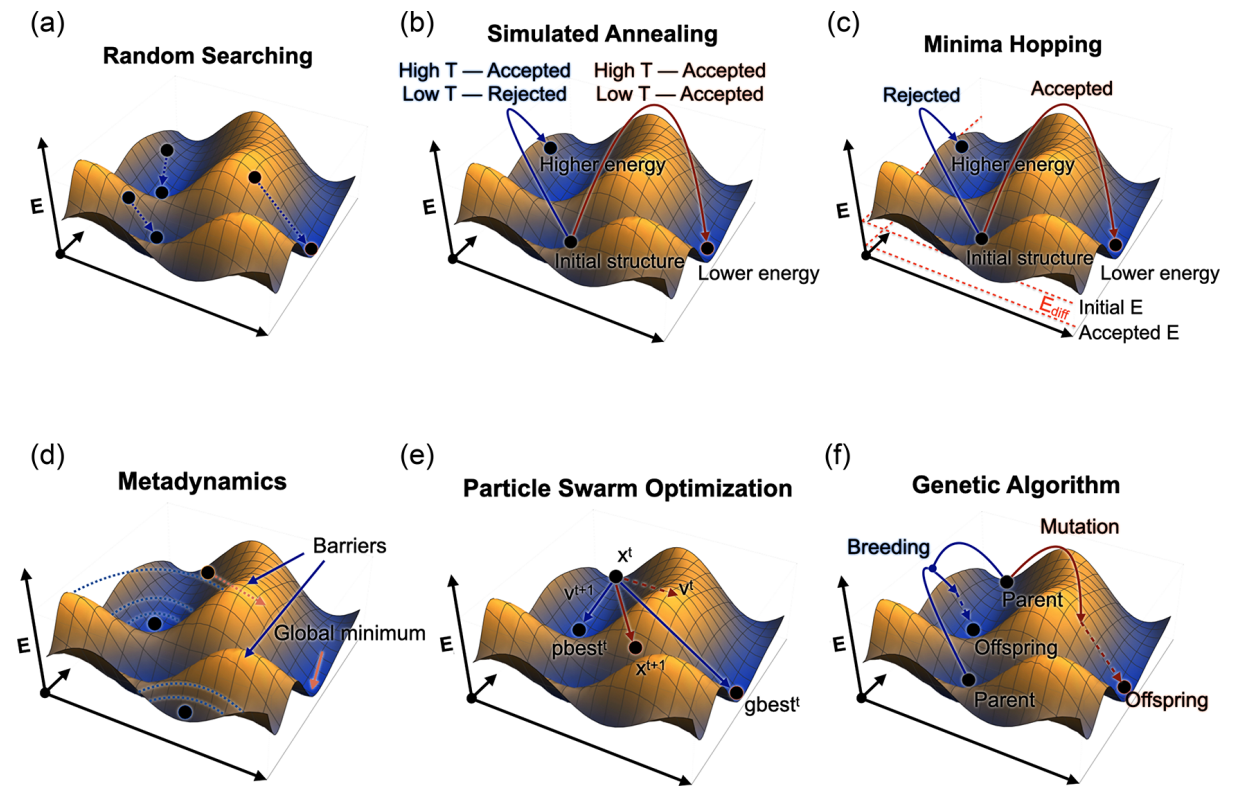
\includegraphics[width=\columnwidth]{figures/optim_figures.png}
                \captionof{figure}{Schematic explanation of various crystal structure prediction methods, by Falls et al. \cite{Falls2020}}\medskip

Each method has its own advantages and inconvenients, and has been probed for the generation of configurations. Thus, there is still no consensus for a specific method, as techniques can be better in some cases. \vspace{1em}

This report, based on the publication from Naden Robinson et al. \cite{original}, tackles the application of another generalized optimization algorithm (Particle Swarn Optimization) for the purposes of potential energy surfaces exploration and the determination of the optimized geometry for extreme conditions. The study is based on the exploration of ammonia-water mixtures present inside planets of our solar system (especially Uranus and Neptune). In these mantles, there exists some particularly harsh conditions, that are not existing in our planet: indeed, high temperatures and pressure can be reached; thus accessing zones of the phase diagram of this mixture that were never explored previously. Furthermore, it is almost impossible in this case to use experiments in the first place to have first guesses, and as we have no clue about any stoechiometry, symmetry or parameters, sampling the entire potential energy surface would be very computationally expensive. Those reasons also exclude many of the above methods, that would require an initial configuration, and/or a clear final destination. As a matter of consequence, using a smart optimization technique is, of course, of high importance.

%Faire une introduction sur la nécessité de devoir générer des configurations par la théorie dans le cas de conditions expérimentales exotiques (on ne peut pas se baser sur des expériences précédentes car il n'y en a pas lol)
\section*{Particle Swarn Optimization}
\subsection*{Theoretical background}
Particle Swarm Optimization (also called PSO) is a population-based optimization algorithm that simulates the social behavior of birds or insects, such as flocking or swarming.   \cite{PhysRevB.82.094116,WANG20122063}
\begin{itemize}
\itemsep0em
    \item Generation of one random structure per symmetry (avoids unnecessary calculations)
    \item Local optimization of every structure
    \item Exclusion of similar structures
    \item Generation of new structures by PSO
    \item Repeating steps 2, 3 and 4 until convergence is reached
    \item Returns the configuration with the lowest energy
\end{itemize}
\bigskip

              \noindent 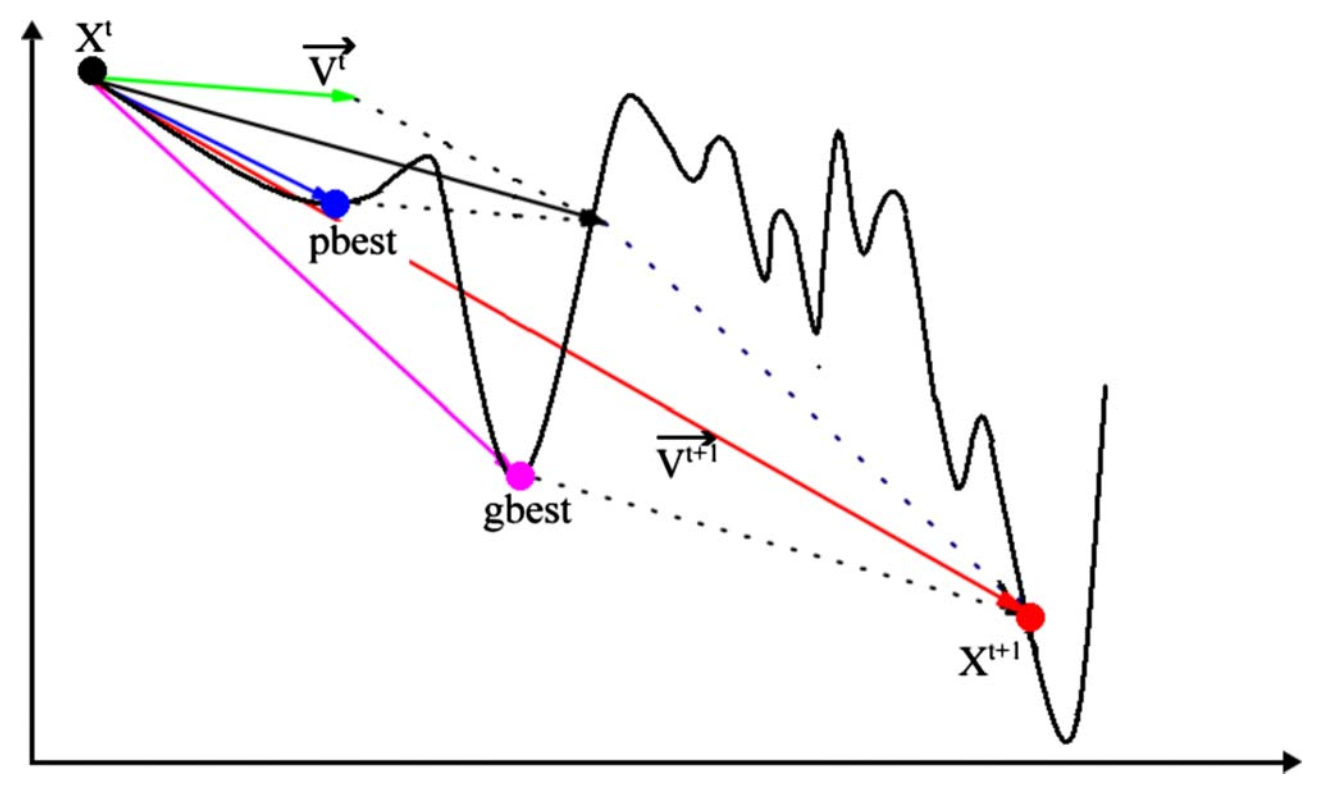
\includegraphics[width=\columnwidth]{figures/PSO.png}
                \captionof{figure}{Schematic explanation of particle swarn optimization, by Wang et al. \cite{PhysRevB.82.094116}}\medskip
\subsection*{Programming PSO, trial over a simple two-dimensional study case}
Usage of the Eggholder function
\section*{Obtained results}
\section*{Comparison to other generation methods}

\section*{Conclusion}
\end{multicols}
\bibliographystyle{bibstyle.bst}
\bibliography{articles}

\end{document}